\chapter{Progetto di \textit{stage}}
    \section{Gestione degli \textit{stage} in SogeaSoft S.r.l.}
    SogeaSoft S.r.l. riconosce il valore strategico degli \textit{stage} curricolari, considerandoli un'opportunità sia per la formazione di potenziali nuovi dipendenti, sia per l'esplorazione di nuove tecnologie e la valutazione critica dei sistemi attualmente in uso. Tali percorsi formativi consentono non solo di trasferire conoscenze e competenze, ma anche di promuovere un'analisi approfondita delle soluzioni tecnologiche adottate dall'azienda, favorendo l'innovazione e l'ottimizzazione dei processi.  

    \vspace{0.2 em}
    Le attività svolte nell'ambito degli \textit{stage} possono includere: 
    \begin{itemize}
        \item l'integrazione di nuove funzionalità nei sistemi esistenti, con l'obiettivo di migliorarne le prestazioni e l'efficienza;
        \item lo studio e lo sviluppo di strumenti autonomi a supporto dei processi di sviluppo o dei prodotti in uso, come ad esempio Swagger, una piattaforma per la documentazione e il testing delle API;  
        \item l'analisi formale di strumenti già utilizzati in azienda, ma impiegati prevalentemente in modo empirico, al fine di standardizzarne e ottimizzarne l’uso;  
        \item la conduzione di attività di monitoraggio sulle \textit{performance} di determinati sistemi, per identificarne eventuali criticità e proporre soluzioni migliorative.  
    \end{itemize}

    \vspace{0.2 em}
    \noindent L'evoluzione tecnologica in SogeaSoft S.r.l. può avvenire attraverso diverse strategie, tra cui l’ampliamento delle funzionalità della \textit{codebase} esistente, l’analisi teorica dello stato dell’arte o la realizzazione di \textit{software} sperimentali, quali \textit{Proof of $Concept_G$} ($PoC_G$) o prodotti già pronti per un utilizzo immediato, come il \textit{Minimum Viable $Product_G$} ($MVP_G$). Nel contesto del mio \textit{stage}, le attività svolte hanno combinato questi approcci, consentendo non solo lo sviluppo di una soluzione concreta, ma anche la produzione di una documentazione tecnica approfondita. Tale metodologia si è rivelata particolarmente efficace per garantire una comprensione strutturata del problema e facilitare eventuali iterazioni successive.  

    \vspace{0.2 em}
    \noindent SogeaSoft S.r.l. attribuisce particolare valore agli \textit{stage}, poiché rappresentano un'opportunità strategica per affrontare una delle sue principali sfide tecnologiche: la migrazione del proprio prodotto da un’architettura $monolitica_G$ a un’architettura a $microservizi_G$, come discusso nella Sezione 1.8. Gli \textit{stage} costituiscono una risorsa vantaggiosa sotto molteplici aspetti: da un lato, permettono di ottimizzare l’investimento in ricerca e sviluppo grazie a costi contenuti; dall’altro, consentono all’azienda di entrare in contatto con prospettive innovative, idee originali e persone non condizionate dai paradigmi consolidati all'interno dell’azienda.  

    \vspace{0.2 em}
    \noindent Un ulteriore fattore determinante nell’impiego di tirocinanti per lo sviluppo di soluzioni innovative è la gestione delle risorse interne. Il personale aziendale è prevalentemente impegnato nel mantenimento e nell’evoluzione dei sistemi attualmente in produzione, rendendo complesso il reindirizzamento delle competenze su progetti sperimentali. L’inserimento di studenti permette di destinare risorse dedicate a iniziative di ricerca e innovazione, garantendo al contempo un processo di trasferimento di conoscenze tra le diverse generazioni di sviluppatori.
    
    \section{Il \textit{software} SAI}
    
    Il tema principale del mio \textit{stage} ha riguardato lo sviluppo e l’evoluzione di SAIonWeb, un \textit{software} basato sul \textit{framework} SAI (Sistema Aziendale Integrato). SAIonWeb è uno strumento progettato per la gestione dei processi aziendali nell’ambito dell’\textit{Enterprise Resource Planning} (ERP). In particolare, il \textit{software} è destinato al settore manifatturiero, con un \textit{focus} specifico sull'industria dell’abbigliamento, supportando l'intero ciclo di vita del prodotto: dalla gestione delle materie prime, alla fase di confezionamento, fino alla distribuzione finale.  

    \vspace{0.2 em}
    \noindent Il \textit{framework} SAI, alla base di SAIonWeb, è caratterizzato da un'architettura monolitica, un modello in cui tutti i componenti del sistema, dall’interfaccia utente alla logica applicativa e alla gestione dei dati, sono strettamente integrati all’interno di un'unica applicazione.  

    \vspace{0.2 em}
    \noindent L'obiettivo del mio stage è stato analizzare il funzionamento di SAI, identificando il dominio applicativo, i \textit{bounded $contexts_G$} e le possibili suddivisioni in microservizi. Il lavoro ha comportato un'attività di studio approfondita dell'architettura esistente, al fine di individuare i servizi che potevano essere estratti e trasformati in unità indipendenti, contribuendo così al processo di migrazione verso SAIonWeb, pensata per adottare un'architettura a microservizi. Inoltre, il progetto ha previsto la valutazione delle scelte progettuali già adottate dai dipendenti, con la possibilità di proseguire il lavoro esistente o, ove necessario, modificarlo per garantire una transizione più efficace e coerente con i principi del \textit{Domain-Driven Design} (DDD). 
    
        \subsection{Funzionalità generali di SAI}
        SAI \textit{Enterprise Resource Planning} (ERP) è un sistema software gestionale progettato per integrare e automatizzare i processi aziendali, consentendo alle organizzazioni di gestire in modo efficiente risorse, dati e operazioni. Questi sistemi offrono un ambiente centralizzato in cui le diverse aree aziendali – dalla produzione alla logistica, dalla contabilità alla gestione delle risorse umane – possono operare in modo coordinato, migliorando la tracciabilità delle informazioni e ottimizzando la produttività.  

        \vspace{0.2 em}
        \noindent SAI è un ERP specificamente sviluppato per il settore dell'abbigliamento, supportando l’intero ciclo di produzione e distribuzione di capi di moda. Le sue funzionalità principali includono:  
        \begin{itemize}
            \item \textbf{Gestione delle materie prime}: monitoraggio degli approvvigionamenti, delle scorte e della qualità dei materiali;
            \item \textbf{Pianificazione della produzione}: organizzazione delle fasi produttive, assegnazione delle risorse e gestione dei tempi di lavorazione;
            \item \textbf{Tracciabilità dei prodotti}: controllo dell’avanzamento di ciascun capo, dalla fase iniziale di lavorazione fino alla distribuzione;
            \item \textbf{Gestione degli ordini e delle vendite}: registrazione degli ordini, gestione delle consegne e fatturazione automatizzata;
            \item \textbf{Logistica e distribuzione}: coordinamento delle spedizioni, gestione dei magazzini e ottimizzazione delle scorte;
            \item \textbf{Integrazione con il sistema contabile}: gestione di pagamenti, bilanci e rendicontazione finanziaria;
            \item \textbf{Monitoraggio delle performance aziendali}: generazione di report analitici e strumenti di business intelligence per supportare il processo decisionale.  
        \end{itemize}

        \vspace{0.2 em}
        \noindent Attraverso queste funzionalità, SAI consente alle aziende del settore moda di migliorare la gestione delle operazioni, ridurre i tempi di produzione e garantire una maggiore efficienza operativa.
        
        \subsection{L'architettura di SAI}
        Il software SAI è caratterizzato da un’architettura monolitica, termine che evoca l’idea di una struttura compatta e unitaria, in cui le varie componenti sono strettamente interconnesse e formano un insieme indivisibile. Nel contesto dell'architettura software, tale espressione indica un sistema in cui tutte le funzionalità sono integrate in un’unica unità di *deployment*, costituendo una struttura unificata in cui ciascun componente dipende dagli altri per garantire il corretto funzionamento dell’intero sistema.  

        Quando si parla di architettura software, ci si riferisce alla struttura fondamentale di un siste ma, comprendente i suoi componenti principali, le interazioni tra essi, i principi di progettazione adottati e il contesto operativo in cui l’applicazione si inserisce.

        Le principali caratteristiche di un’architettura monolitica sono le seguenti:  

        - **Integrazione delle funzionalità in un unico blocco applicativo**: tutte le funzionalità sono raccolte in un’unica entità, che viene distribuita come un blocco indivisibile. Questo implica che ogni modifica apportata a una parte del codice può avere ripercussioni su altre parti del sistema, rendendo complessi gli aggiornamenti e la manutenzione. Di conseguenza, con l’evolversi del progetto, l’accumulo di *debito tecnico* può far sì che il software diventi eccessivamente complesso e difficilmente adattabile a nuove tecnologie.  

        - **Scalabilità verticale**: la scalabilità in un sistema monolitico si ottiene potenziando l’intera applicazione per affrontare un aumento del carico di lavoro. Anche qualora solo alcune funzionalità necessitassero di risorse aggiuntive, l’intero sistema deve essere potenziato, comportando uno spreco di risorse. Non essendo possibile una scalabilità modulare, si tende a duplicare l’intera applicazione per garantire le prestazioni richieste.  

        - **Bassa granularità**: l’architettura monolitica presenta una scarsa separazione delle funzionalità, che risultano strettamente integrate e difficilmente isolabili. Questo limita significativamente la flessibilità del sistema e ostacola l’integrazione di nuovi moduli o tecnologie senza compromettere la stabilità complessiva.  

        L’architettura monolitica del sistema SAI rappresenta una sfida in termini di manutenibilità e adattabilità alle tecnologie moderne, evidenziando la necessità di migrare verso un’architettura a microservizi per migliorare la modularità, la scalabilità e l’agilità del sistema stesso.
        
        L'obiettivo del mio stage è stato quello di fornire una base formale e metodologica al lavoro empirico già avviato da SogeaSoft S.r.l. riguardo alla migrazione verso un'architettura a microservizi, con l’intento di superare i limiti strutturali del sistema attuale e di garantire una maggiore flessibilità e scalabilità in futuro.
        
        L'architettura a microservizi si caratterizza per la natura decentralizzata e per l’unità di esecuzione non strettamente dipendente dalle altre componenti del sistema. I microservizi comunicano tra loro tramite *network*, configurandosi come una forma di sistema distribuito. Un principio fondamentale di questa architettura è il *deploy indipendente*, che si realizza garantendo un basso grado di accoppiamento (*loose coupling*) tra i servizi.  

        Una caratteristica distintiva dei microservizi è l’assenza di un database condiviso: ogni servizio mantiene il proprio database locale e, qualora necessiti di accedere ai dati di un altro servizio, deve effettuare una richiesta esplicita. Questo approccio consente di definire con precisione quali dati sono visibili e quali rimangono nascosti, favorendo il deployment indipendente.  

        Per garantire un’architettura efficace, i microservizi devono rispettare due principi fondamentali:  
        \begin{itemize}
            \item Basso accoppiamento (Loose coupling): Un microservizio è considerato debolmente accoppiato se è possibile modificarlo senza la necessità di aggiornare altri servizi correlati. Questo principio favorisce la manutenibilità e l'evoluzione del sistema, evitando effetti a cascata.
            \item - **Alta coesione funzionale (High cohesion)**: Ogni microservizio dovrebbe avere un unico e ben definito scopo, raggruppando le funzionalità in modo tale da minimizzare le modifiche in punti distinti del sistema. 
        \end{itemize}

        Un ulteriore concetto rilevante è l’*information hiding*, ovvero la separazione delle parti di codice soggette a frequenti cambiamenti da quelle più statiche. L’approccio suggerito prevede di nascondere il maggior numero possibile di dettagli interni, esponendo solo ciò che è strettamente necessario, in modo da mantenere il sistema più stabile e flessibile.  

        Inoltre, secondo i principi del Domain-Driven Design ogni microservizio dovrebbe:  
        - Incapsulare la *domain knowledge* e l’*abstract knowledge* dai clienti, concentrandosi sulla propria responsabilità specifica.  
        - Definire l’architettura e i confini in base al rispettivo dominio anziché all’intero sistema, garantendo una chiara separazione delle responsabilità e una gestione modulare delle funzionalità.  

        Questo approccio consente di costruire sistemi resilienti e scalabili, in cui l'evoluzione tecnologica può avvenire in modo graduale e senza compromettere l'integrità complessiva del sistema.

        \begin{figure}[H]
            \centering
            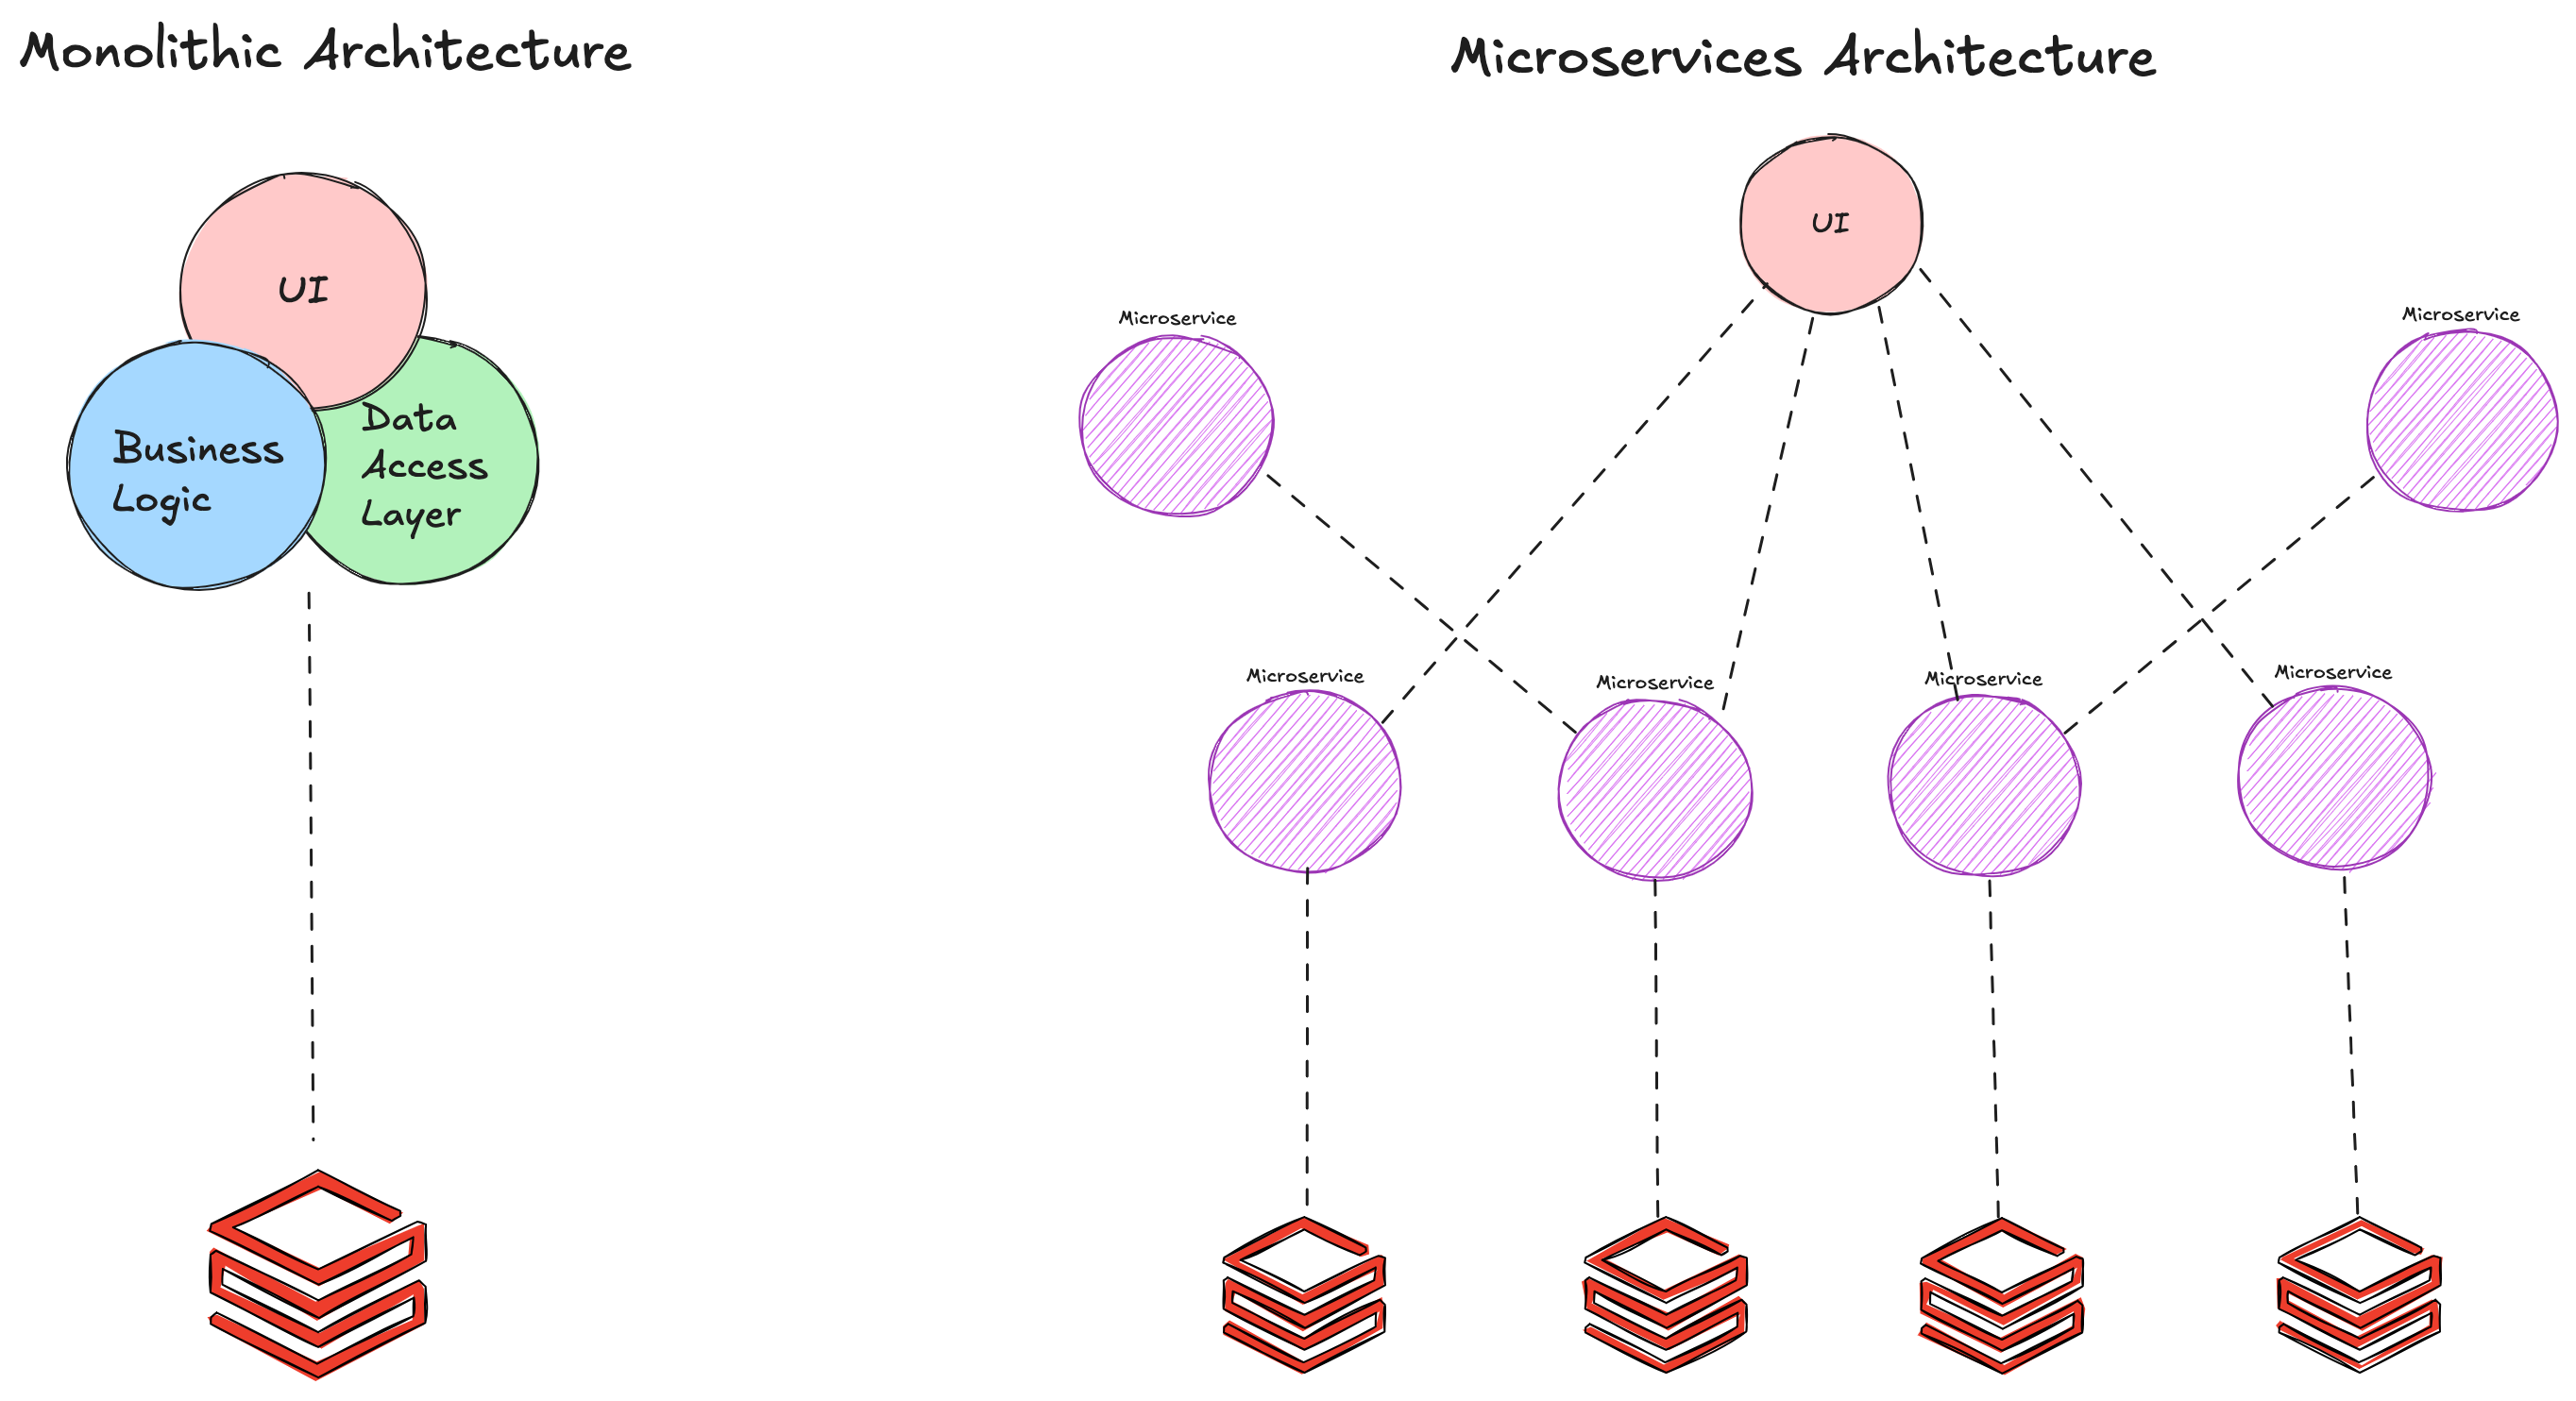
\includegraphics[width=0.9\linewidth]{BCS-Tessi/images/Monolith-Microservices.png}
            \caption[Differenza tra un sistema monolitico e uno a microservizi]{Differenza tra un'architettura monolitica e un'architettura basata su microservizi.}
            \label{fig:monolith-vs-microservices}
        \end{figure}

        \subsection{La migrazione}
        SogeaSoft S.r.l. desidera dunque migrare da un'architettura monolitica a un'architettura a microservizi. Già diverse attività sono state attuate, il mio compito è stato quello di porre una base teorica più solida ed eventualmente confermare o confutare le scelte implementate, nonché prendere nuove decisioni riguardo a particolari casi d'uso nel mio progetto specifico di stage. 
        SogeaSoft S.r.l. ha intrapreso un percorso di migrazione da un'architettura monolitica a un'architettura a microservizi, con l'obiettivo di migliorare la scalabilità, la manutenibilità e la flessibilità del proprio software gestionale. Sebbene diverse attività siano già state implementate in questa direzione, il mio compito durante il progetto di stage è stato quello di consolidare le basi teoriche dell'approccio adottato, analizzando criticamente le scelte progettuali già effettuate. In particolare, ho avuto il compito di confermare o confutare l'adeguatezza delle soluzioni implementate e di prendere nuove decisioni rispetto a specifici casi d'uso legati al progetto assegnato.  

        Uno degli elementi centrali della migrazione riguarda l'introduzione di una componente denominata **MicroService-Middleware**, implementata come un *Anti-Corruption Layer* (ACL). In ambito architetturale, un ACL è un modello progettuale che funge da interfaccia tra sistemi legacy e nuove componenti, prevenendo la propagazione di modelli obsoleti o incoerenti nelle parti più moderne del sistema. Nel contesto di SogeaSoft, il MicroService-Middleware si occupa di ricevere le richieste provenienti dall'ERP monolitico e, tramite un **Message Broker**, instradare tali richieste verso il microservizio appropriato. Il Message Broker, infatti, svolge il ruolo di intermediario per lo scambio di messaggi tra componenti software, garantendo una comunicazione asincrona ed efficiente tra i vari microservizi.  

        Ogni microservizio, una volta attivato, esegue la funzione richiesta in modo autonomo e indipendente, restituendo l’esito tramite lo stesso meccanismo di messaggistica. Per rendere accessibili le funzionalità esposte dai microservizi, l'azienda ha implementato una **WebAPI Gateway**, che rappresenta un punto di accesso centralizzato alle API dei vari servizi. La WebAPI Gateway consente di aggregare e orchestrare le chiamate ai microservizi, creando un'interfaccia unificata verso l'utente finale.  

        Grazie a questa architettura, il sistema è in grado di supportare una **Single Page Application (SPA)**, un tipo di applicazione web che carica una singola pagina HTML e aggiorna dinamicamente il contenuto man mano che l'utente interagisce. Questo approccio garantisce un'esperienza utente più fluida e interattiva, riducendo i tempi di caricamento e ottimizzando le performance dell'applicazione.  

        L'adozione di queste soluzioni riflette la volontà dell'azienda di superare le limitazioni dell'architettura monolitica, garantendo maggiore modularità e adattabilità alle nuove tecnologie, pur mantenendo la continuità dei servizi già in essere.
        
        
    \section{Obiettivi del progetto di \textit{stage}}
        \subsection{Obiettivi aziendali}
        Scriverò degli obiettivi dello \textit{stage}, introducendo il desiderio dell'azienda di migrazione verso un'architettura a microservizi. Racconterò delle motivazioni in modo più approfondito, e riporterò gli obiettivi obbligatori, desiderabili e opzionali decisi all'inizio dell'attività di \textit{stage}.
        \subsection{Vincoli}
        Descriverò i vincoli relativi all'attività di \textit{stage}, saranno temporali e tecnologici. 

    \section{Metodo di Lavoro}
        \subsection{Piainificazione}
        Riporterò il piano di lavoro iniziale e descriverò la suddivisione delle ore, la pianificazione temporale delle attività e il tempo di perseguimento degli obiettivi di avanzamento. 
        \subsection{Modello di sviluppo}
        Rifacendomi alla sezione 1.4, racconterò quanto effettivamente il modello di sviluppo adottato da SogeaSoft S.r.l. sia stato applicato durante il mio \textit{stage} rispetto agli accordi iniziali. 
        \subsection{Strumenti}
        Descriverò, gli strumenti utilizzati a supporto della mia esperienza di \textit{stage}, tra cui gli appunti, le presentazioni, i \textit{report} etc. 
        \subsection{Revisioni di Progresso}
        Riporterò tutte le occasioni di confronto con il \textit{tutor}, le revisioni ufficiali del lavoro svolto ed altri eventuali strumenti messi a disposizione per il monitoraggio del progresso. 
    \section{Motivazioni della scelta}
    Descriverò le motivazioni della mia personale scelta riguardo questo particolare progetto di \textit{stage}, raccontando perché l'ho scelto rispetto ad altri. Descriverò anche gli obiettivi e le aspettative personali, che riprenderò nella sezione 4.1.2
    
        